\documentclass{standalone}
\usepackage[ascii]{inputenc}
\usepackage{tikz}

\usetikzlibrary{patterns}

\begin{document}

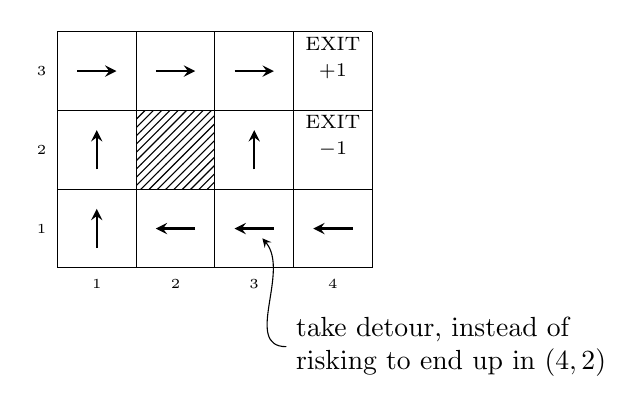
\begin{tikzpicture}[>=stealth]
\draw (0,0) grid (4,3);
\draw [pattern=north east lines] (1,1) rectangle (2,2);
\node at (0.5,-0.2) {\tiny 1};
\node at (1.5,-0.2) {\tiny 2};
\node at (2.5,-0.2) {\tiny 3};
\node at (3.5,-0.2) {\tiny 4};
\node at (-0.2,0.5) {\tiny 1};
\node at (-0.2,1.5) {\tiny 2};
\node at (-0.2,2.5) {\tiny 3};
\node at (3.5,1.85) {\scriptsize EXIT};
\node at (3.5,2.85) {\scriptsize EXIT};
\node at (3.5,1.5)  {\scriptsize $-1$};
\node at (3.5,2.5)  {\scriptsize $+1$};
\draw [->,thick] (0.5,0.25) -- (0.5,0.75);
\draw [->,thick] (0.5,1.25) -- (0.5,1.75);
\draw [->,thick] (0.25,2.5) -- (0.75,2.5);
\draw [->,thick] (1.75,0.5) -- (1.25,0.5);
\draw [->,thick] (1.25,2.5) -- (1.75,2.5);
\draw [->,thick] (2.75,0.5) -- (2.25,0.5);
\draw [->,thick] (2.5,1.25) -- (2.5,1.75);
\draw [->,thick] (2.25,2.5) -- (2.75,2.5);
\draw [->,thick] (3.75,0.5) -- (3.25,0.5);
\node[align=left] (nL) at (5, -1) {take detour, instead of \\ risking to end up in $(4,2)$};
\node (nA) at (2.5, 0.5) {};
\draw (nL) edge [->, out=180, in=310] (nA);
\end{tikzpicture}

\end{document}
